In this chapter, we describe our proposal of using genetic improvement, \textit{i.e. the Gin toolbox}, for software energy efficiency. To do that, we investigate in which extent three fitness functions can reduce energy consumption.
Then, Next steps for integrating code refactoring to the gin toolbox are also provided in Section~\ref{sec:nextSteps} of Chapter~\ref{ch:conclusion}. %this preliminary work is to integrate

\section{Tactics for reducing energy consumption}\label{sec:tactics}

%GI ... fitness function
When using the Gin tool to improve a method within a program, we need to determine the appropriate fitness function. This function will guide the optimization process, ultimately yielding an improved version of the selected method for the program.
%RQ2.1
Based on our research question \textbf{RQ2.1}, we selected two types of fitness functions. These are:

% Single criteria fitness function
  %Tactic 1: Minimising time execution 
  %Minimising memory consumption
% Multi criteria fitness function
  % Minimising time execution and minimising memory consumption
  
\begin{enumerate}
    \item Single criteria fitness function
    \begin{itemize}
        \item \textbf{Tactic 1:} Minimize Execution Time
            \begin{itemize}
             \item \textbf{Objective:} Reduce the execution time of the program. Using this tactic, the 'gin' tool will generate an optimal patch that corresponds to the shortest execution time. This approach ensures that the code associated with the optimal patch not only compiles successfully but also enhances the program's execution time performance.
             \end{itemize}

        \item \textbf{Tactic 2:} Minimize Memory Consumption
            \begin{itemize}
            \item \textbf{Objective:} Decrease the memory usage of the program. With this tactic, the 'gin' tool will produce an optimal patch leading to reduced memory consumption. This method ensures that the code linked with the optimal patch compiles successfully and improves the program's memory consumption performance. Gin’s default \texttt{LocalSearch} Java class was primarily designed for execution time minimization. Given our specific objective of memory consumption minimization, we made modifications to the \texttt{LocalSearch} class.(see Appendix~\ref{sec:LocalSearch_Memory} for more details of updated version of the \texttt{LocalSearch} class)
            \end{itemize}
    \end{itemize}
    \item Multi criteria fitness function
    \begin{itemize}
        \item \textbf{Tactic 3}: Minimising Execution Time and minimising Memory Consumption.
        \begin{itemize}
            \item \textbf{Objective:} Reduce both the execution time and the memory usage of the program concurrently. Using this tactic, the 'gin' tool will generate an optimal patch that strikes a balance between minimizing execution time and memory consumption. This strategy ensures that the code associated with the optimal patch compiles successfully and offers a harmonized improvement in both the program's execution time and memory consumption performance. We adapted Gin’s default \texttt{LocalSearch} Java class to minimize both execution time and memory consumption together (see Appendix~\ref{sec:LocalSearch_Time_Memory} for more details of updated version of the \texttt{LocalSearch} class). To achieve this, a unique scoring system was devised where both the execution time and memory usage for each patch are normalized and summed. This aggregated score acts as the objective function, with the goal being its minimization. Consequently, a lower score indicates better performance in terms of time and memory. Throughout its iterations, the \texttt{LocalSearch} class tests various patches on the source code, selecting and retaining the one that produces the lowest score, thus ensuring efficient code performance.
            \end{itemize}
    \end{itemize}
\end{enumerate}

\section{Experimental Study Design }
%In this section, we detail the experiments conducted using the Gin tool to obtain optimized versions of selected programs. 
As mentioned, the evaluations using Gin were based on single-criteria fitness functions such as \textit{minimizing execution time} and \textit{minimizing memory consumption}, as well as a multi-criteria fitness function related to \textit{minimizing execution time and memory consumption} at the same time. 

\vspace{.5em}
We selected three programs for our experiments: \textit{Triangle}, \textit{Greatest Common Divisor (GCD)}, and \textit{Rectangle}. 

\vspace{.5em}
After the three programs were optimized with Gin, we collect data of energy consumption for the original and optimized versions of these programs by using \textit{JoularJX}.
%we performed two additional experiments for each program to determine the energy consumption of both the original and optimized versions using joularJX. 
%These experiments aimed to compare the energy consumption of the optimized versions with that of their original versions. 
Then we compare data gathered from the optimised and original versions of java programs. 
%if any improvement in terms of energy consumption 
To determine any significant difference between the data, we used the \texttt{Wilcoxon} statistical Test because the data distribution is non-normal. 

\vspace{.5em}
From these results, we will be able to address \textbf{RQ2.1}, which will help us determine whether the optimized version of the program, using the gin tool, has a significant impact on the reduction of energy consumption.

\subsection{Experimental Procedure to use Gin}
%\subsubsection{Experimental procedures}
To run our experiments, we sequentially executed the following steps:

\begin{enumerate}

\item \textbf{Prerequisites:} Gin requires:
\begin{itemize}
\item JDK 17
\item Gradle (tested with version 8.0.2)
\item A number of dependencies, which can be downloaded manually or via Gradle (recommended)
\item For Maven projects: make sure the Java version is set to the same version as Gin's.
\end{itemize}

\item \textbf{Clone the Repository:} Start by cloning the repository using the following command:

\begin{verbatim}
git clone https://github.com/gintool/gin.git
\end{verbatim}

\item \textbf{Navigate to the examples Directory:} Change the directory to the project folder:
\begin{verbatim}
cd gin/examples/triangle
\end{verbatim}

\item \textbf{Compile the java class file (\eg TriangleTest.java) :} Compile the TriangleTest.java program by running the following command:
\begin{verbatim}
javac -cp /usr/share/java/junit4.jar:. TriangleTest.java
\end{verbatim}

\item \textbf{Navigate to the gin Directory:} Change the directory to the gin folder:
\begin{verbatim}
cd ../../
\end{verbatim}

\item \textbf{Build using gradle (alternatively import into any IDE, such as IntelliJ) :}
\begin{verbatim}
gradle build
\end{verbatim}

This will build and test Gin, and also create a fat jar at build/gin.jar containing all required dependencies.

Note: If the provided build command will not work use the following command below:
\begin{verbatim}
./gradlew clean build -x test copyToLib
\end{verbatim}

This will ensure a clean build by removing any existing build artifacts, compiles the source code, skips test execution, and then executes the custom copyToLib task, which carries out additional project-specific actions defined in the build script and also create a fat jar at build/gin.jar containing all required dependencies.


\item \textbf{Execute the local search on a simple example:}
\begin{verbatim}
java -jar build/gin.jar -f examples/triangle/Triangle.java -m 
"classifyTriangle(int,int,int)"
\end{verbatim}

Note: If the provided command for Running a Simple Example will not able to work, follow the below informations and execute the commands:
\begin{verbatim}
java -cp build/gin.jar:lib/junit-vintage-engine-5.9.2.jar gin.LocalSearch -f
examples/triangle/Triangle.java -m "classifyTriangle(int,int,int)"
\end{verbatim}
Note: In this command specified the location of the necessary JAR files.
\end{enumerate}


\section{Experimental Results using Gin}

\subsection{Triangle Program}
\label{sec:Triangle}
 
The \textit{Triangle} code classifies triangles, given their side lengths, into one of four categories: invalid, equilateral, isosceles, or scalene. By sorting the input sides and analyzing their relationships, the program identifies and returns the type of triangle.

\vspace{.5em}
Specifically, our goal was to enhance the performance of the \texttt{classifyTriangle} method within the \textit{Triangle} program (see Appendix~\ref{sec:triangle}). We targeted the three fitness criteria mentioned in Section~\ref{sec:tactics} to optimize the triangle code using Gin.
Then optimized and original versions of the \textit{Triangle} code are compare in terms of their energy consumption. 


\subsubsection{Single criteria Fitness Function: Tactic 1(Minimizing execution time)}

For the \textit{triangle} java code, we minimize its execution time by using the Gin toolbox. Figure~\ref{fig:Optimised program file of Triangle 1} shows the execution of Gin on the \textit{triangle} code. As seen, it provides information about each step of the local search execution. It started with a summary of the file and method being analyzed, followed by reporting the original execution time of the method. As Figure~\ref{fig:Optimised program file of Triangle 1} shows, the execution time for the original version of the \textit{triangle} java code was 1636120217ns.

%\vspace{1.5em}
\begin{figure}[ht!]
  \centering
  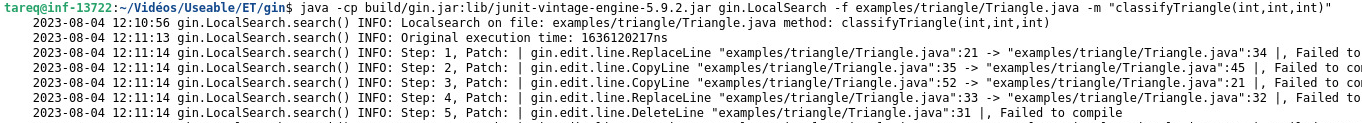
\includegraphics[width=1\textwidth]{img/Triangle_Experiment_output_1.png}
  \caption{Command line output: Optimized Triangle Java program with Gin tool.}
  \label{fig:Optimised program file of Triangle 1}
\end{figure}

\vspace{.5em}
For each step, the output indicated the patch being applied to the code. If a patch fails to compile, it means that the modified code could not be compiled successfully and this patch is discarded.If the patched code is complied and passes all provided tests, the execution time is calculated and showed if it better to previous version of code.

\begin{figure}[ht!]
  \centering
  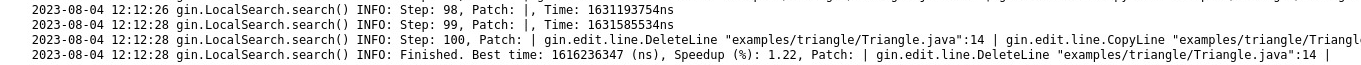
\includegraphics[width=1\textwidth]{img/Triangle_Experiment_output_2.png}
  \caption{Command line output: Optimized Triangle Java program with Gin tool.}
  \label{fig:Optimised program file of Triangle 2}
\end{figure}

\vspace{.5em}
The local search algorithm continued for a specified number of steps (condition for stopping  the Gin process), which was set to 100 by default (see Figure \ref{fig:Optimised program file of Triangle 2}). Throughout the process, different patches were generated and evaluated, aiming to find an optimized version of them.By examining the output, we could identify the patches that resulted in successfully compiled code and improved execution time. At the end of the process, a brief summary was provided to give an overview of the optimization results. Best time(Lowest execution time): 1616236347 (ns), Speedup (\%): 1.22.

\vspace{.5em}
Figure \ref{fig:Optimised program file of Triangle}
shows that the optimized code was generated. The figure displays the Optimised program file of the Triangle program in blue, representing the code that has been improved for better performance. Conversely, the green color represents the original program file of the Triangle program, which is the code in its initial state without any optimization.

\begin{figure}[ht!]
  \centering
  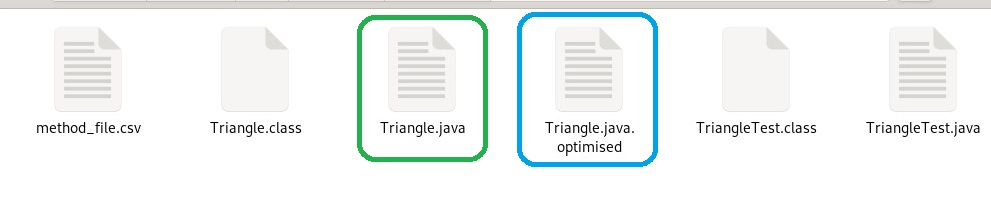
\includegraphics[width=.49\textwidth]{img/Triangle_Experiment_output.jpg}
  \caption{Optimised program file of Triangle}
  \label{fig:Optimised program file of Triangle}
\end{figure}



\subsubsection{Single criteria Fitness Function: Tactic 2(Minimizing memory consumption)}

For the \textit{triangle} java code, we minimize its memory consumption by using the Gin toolbox. Figure~\ref{fig:MC_2} shows the execution of Gin on the \textit{triangle} code. As seen, it provides information about each step of the local search execution. It started with a summary of the file and method being analyzed, followed by reporting the original memory consumption of the method. As Figure~\ref{fig:MC_2} shows, the memory consumption for the original version of the \textit{triangle} java code was 28 Mbytes.

\begin{figure}[htbp]
  \centering
  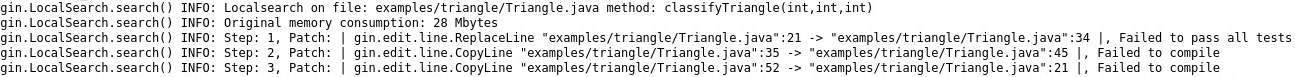
\includegraphics[width=1\textwidth]{img/Triangle_MC_2.png}
  \caption{Command line output: Memory Consumption Optimized Triangle Java program with Gin tool.}
  \label{fig:MC_2}
\end{figure}

\vspace{5em}
For each step, the output indicated the patch being applied to the code. If a patch fails to compile, it means that the modified code could not be compiled successfully and this patch is discarded. If the patched code is complied and passes all provided tests, the memory consumption is calculated and showed if it better to previous version of code.

\vspace{.5em}
The local search algorithm continued for a specified number of steps (condition for stopping  the Gin process), which was set to 100 by default (see Figure \ref{fig:MC_1}). Throughout the process, different patches were generated and evaluated, aiming to find an optimized version of them. By examining the output, we could identify the patches that resulted in successfully compiled code and improved memory consumption. At the end of the process, a brief summary was provided to give an overview of the optimization results. Best memory consumption: 22 Mbytes, Memory Consumption Reduction: 21.43\%.

\begin{figure}[htbp]
  \centering
  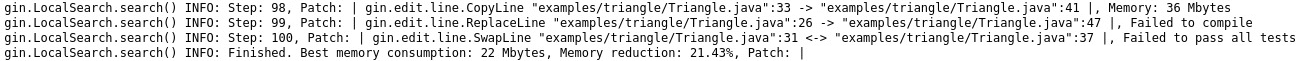
\includegraphics[width=1\textwidth]{img/Triangle_MC_1.png}
  \caption{Command line output: Memory Consumption Optimized Triangle Java program with Gin tool.}
  \label{fig:MC_1}
\end{figure}

\vspace{1em}
Finally, in the same directory where the original Triangle program is, the optimized code of Triangle program for memory consumption was generated based on the best patch that consumed the lowest memory.

\subsubsection{Multi criteria Fitness Function: Tactic 3(Minimizing execution time and memory consumption)}

For the \textit{triangle} java code, we minimize its execution time and memory consumption together by using the Gin toolbox. Figure~\ref{fig:EC_MC_1} shows the execution of Gin on the \textit{triangle} code. As seen, it provides information about each step of the local search execution. It started with a summary of the file and method being analyzed, followed by reporting the original execution time and memory consumption of the method. As Figure~\ref{fig:EC_MC_1} shows, the execution time and memory consumption for the original version of the \textit{triangle} java code was 1773092415 ns and 30 Mbytes.

\begin{figure}[htbp]
  \centering
  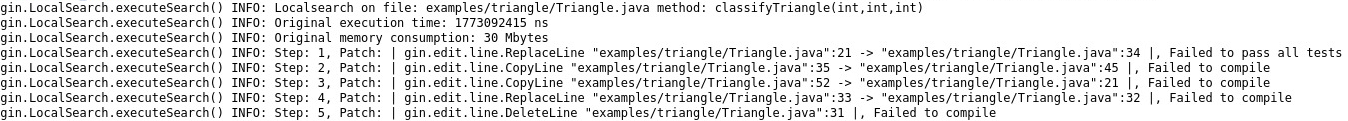
\includegraphics[width=1\textwidth]{img/Triangle_ET_MC_1.png}
  \caption{Command line output: Execution time and Memory Consumption Optimized Triangle Java program with Gin tool.}
  \label{fig:EC_MC_1}
\end{figure}

\vspace{.5em}
For each step, the output indicated the patch being applied to the code. If a patch fails to compile, it means that the modified code could not be compiled successfully and this patch is discarded.If the patched code is complied and passes all provided tests, the execution time and memory consumption are calculated and showed if it better to previous version of code.

\vspace{.5em}
The local search algorithm continued for a specified number of steps (condition for stopping  the Gin process), which was set to 100 by default (see Figure \ref{fig:Ec_MC_2}). Throughout the process, different patches were generated and evaluated, aiming to find an optimized version of them. By examining the output, we could identify the patches that resulted in successfully compiled code and improved execution time and memory consumption together. At the end of the process, a brief summary was provided to give an overview of the optimization results. Best time(Lowest execution time): 1751420953 (ns), Speedup (\%): 1.22, Best memory consumption: 26 Mbytes, Memory reduction: 13.33\%.

\begin{figure}[htbp]
  \centering
  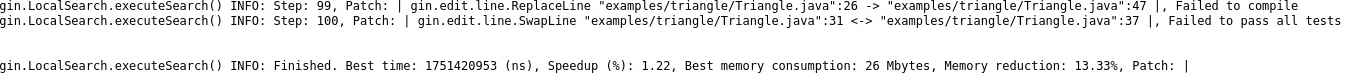
\includegraphics[width=1\textwidth]{img/Triangle_ET_MC_2.png}
  \caption{Command line output: Execution time and Memory Consumption Optimized Triangle Java program with Gin tool.}
  \label{fig:Ec_MC_2}
\end{figure}

\vspace{1em}
Finally, in the same directory where the original Triangle program is, the optimized code of Triangle program for execution time and memory consumption together was generated. This optimization was based on the best patch, which yielded the lowest memory consumption and lowest execution time.

\vspace{-10pt}
\subsection{Greatest Common Divisor(GCD) and Rectangle Program}

The \textit{GCD} Program computes the greatest common divisor (GCD) for three input integers. The fundamental purpose of this program is to determine the largest integer that can evenly divide all three numbers without leaving a remainder. To achieve this, the program utilizes the \texttt{findGCD} method.

\vspace{.5em}
The \textit{Rectangle} program categorizes a four-sided polygon based on its side lengths into one of three classifications: square, rectangle, or invalid shape. By evaluating the dimensions of the given sides, the program discerns the type of quadrilateral. If all four sides are the same length, it is identified as a square. If the opposite sides are equal, it is recognized as a rectangle. Conversely, if any side is non-positive or if the lengths don't fit the criteria for a square or rectangle, the shape is labeled as invalid. To achieve this, the program utilizes the \texttt{classifyRectangle}.

\vspace{.5em}
Specifically, our goal was to enhance the performance of the \texttt{findGCD} and \texttt{classifyRectangle} method within the \textit{GCD} and \textit{Rectangle} program (see Appendix~\ref{sec:GCD} and ~\ref{sec:rectangle}). We targeted the three fitness criteria mentioned in Section~\ref{sec:tactics} to optimize the triangle code using Gin. Then optimized and original versions of the \textit{GCD} and \textit{Rectangle} code are compare in terms of their energy consumption.

\vspace{.5em}
To optimize the two programs(\textit{GCD} and \textit{Rectangle}), using the Gin tool, we followed the same procedures as described for the \textit{Rectangle} program in Section~\ref{sec:Triangle}.

%In this section, we outline our experimental process designed to optimize the "Greatest Common Divisor (GCD)" Java program. Our primary focus was on enhancing the performance of the "findGCD" method within the program. We evaluated the optimization based on three distinct fitness criteria: "Execution Time," "Memory Consumption," and a combined criterion, "Combined Execution Time and Memory Consumption."

%\vspace{.5em}
%To initiate the experiment, we chose the "Greatest Common Divisor (GCD)\footnote{\url{https://gitlabev.imtbs-tsp.eu/sticamsud/enact-internship-2023/-/blob/main/Code/gin/Version_one_Execution_Time/gin/examples/GCD/GCD.java}}" program as our target program. This program's main function is to compute the greatest common divisor (GCD) of three provided integers. The `findGCD` method accepts these integers as parameters and returns their GCD in an efficient manner. Our experiments were based on the previously mentioned fitness criteria. The overarching goal was to bolster the program's efficiency by reducing its execution time, memory consumption, and a balance of both. To achieve these improvements, we used Gin's local search algorithm.

%\subsubsection{Single criteria Fitness: Execution time}

%In this experiment, our objective was to enhance the performance of the "findGCD" method within the "GCD" Java program. Our primary focus was to minimize its execution time. To achieve this, the program was executed using a specified command, and we applied Gin’s local search algorithm.

%\subsubsection{Experimental procedures}
%\begin{enumerate}

%\item \textbf{Prerequisites:} Gin requires:
%\begin{itemize}
%\item JDK 17
%\item Gradle (tested with version 8.0.2)
%\item A number of dependencies, which can be downloaded manually or via Gradle (recommended)
%\item For Maven projects: make sure the Java version is set to the same version as Gin's.
%\end{itemize}

%\item \textbf{Clone the Repository:} Start by cloning the repository using the following command:

%\begin{verbatim}
%git clone https://github.com/gintool/gin.git
%\end{verbatim}

%\item \textbf{Navigate to the examples Directory:} Change the directory to the project folder:
%\begin{verbatim}
%cd gin/examples/GCD
%\end{verbatim}

%\item \textbf{Compile the GCDTest.java file:} Compile the GCDTest.java program by running the following command:
%\begin{verbatim}
%javac -cp /usr/share/java/junit4.jar:. GCDTest.java
%\end{verbatim}

%\item \textbf{Navigate to the gin Directory:} Change the directory to the gin folder:
%\begin{verbatim}
%cd ../../
%\end{verbatim}

%\item \textbf{Build using gradle (alternatively import into any IDE, such as IntelliJ) :}
%\begin{verbatim}
%gradle build
%\end{verbatim}

%This will build and test Gin, and also create a fat jar at build/gin.jar containing all required dependencies.

%Note: If the provided build command will not work use the following command below:
%\begin{verbatim}
%./gradlew clean build -x test copyToLib
%\end{verbatim}

%This will ensure a clean build by removing any existing build artifacts, compiles the source code, skips test execution, and then executes the custom copyToLib task, which carries out additional project-specific actions defined in the build script and also create a fat jar at build/gin.jar containing all required dependencies.


%\item \textbf{Execute (running Gin's local search on a simple example) by running the following command:}
%\begin{verbatim}
%java -jar build/gin.jar -f examples/GCD/GCD.java -m 
%"findGCD(int,int,int)"
%\end{verbatim}

%Note: If the provided command for Running a Simple Example will not able to work, follow the below informations and execute the commands:
%\begin{verbatim}
%java -cp build/gin.jar:lib/junit-vintage-engine-5.9.2.jar gin.LocalSearch -f 
%examples/GCD/GCD.java -m "findGCD(int,int,int)"
%\end{verbatim}
%Note: In this command specified the location of the necessary JAR files.
%\end{enumerate}

%\subsubsection{Experimental Results and Analysis:}

%This section presents the experimental results and analysis of the optimization experiment conducted to achieve an optimized GCD Java program. The focus of the optimization was specifically on improving the "findGCD" method within the program, utilizing the Gin tool.

%\begin{figure}[htbp]
  %\centering
  %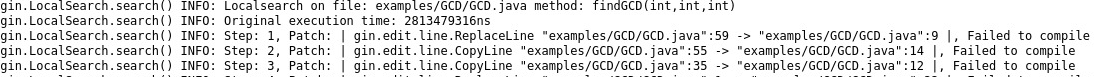
\includegraphics[width=1\textwidth]{img/GCD_ET_1.png}
  %\caption{Command line output:  Execution time Optimized GCD Java program with Gin tool.}
  %\label{fig:GCD_ET_1}
%\end{figure}


%The output(figure \ref{fig:GCD_ET_1}) of the program provided information about each step of the local search process. It started with a summary of the file and method being analyzed, followed by reporting the original execution time of the method.The  Original execution time was 2813479316 ns.

%\begin{figure}[htbp]
  %\centering
  %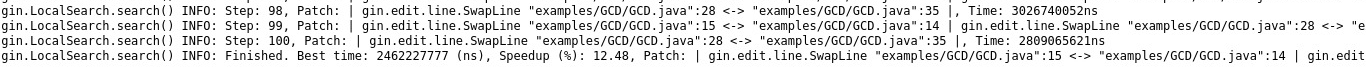
\includegraphics[width=1\textwidth]{img/GCD_ET_2.png}
 %\caption{Command line output:  Execution time Optimized GCD Java program with Gin tool.}
  %%\label{fig:GCD_ET_2}
%\end{figure}


%By examining the output(figure \ref{fig:GCD_ET_2}), we could able to identify the patches that resulted in successfully compiled code and improved execution time performance. The goal was to find the fastest code that passed all provided tests. At the end of the process, a brief summary was provided to give an overview of the optimization results. Best time(Lowest execution time): 2462227777 (ns), Speedup (\%): 12.48.

%\begin{figure}[htbp]
  %\centering
  %
\includegraphics[width=.7\textwidth]{img/GCD_ET_Folder.png}
  %\caption{Optimised program file of GCD program}
  %\label{fig:Optimised program file of GCD program}
%\end{figure}


%In Figure \ref{fig:Optimised program file of GCD program}, the directory where the optimized code was generated is specified. The figure displays the Optimised program file of the GCD program in blue, representing the code that has been improved for better performance. Conversely, the green color represents the original program file of the Triangle program, which is the code in its initial state without any optimization. This color distinction helps visually differentiate between the optimized and original versions of the code.

%\subsubsection{Single criteria Fitness: Memory Consumption}

%In our experiment, we aimed to optimize the memory consumption of the ``findGCD'' method in the ``GCD'' Java program using Gin's local search algorithm. Gin's default \texttt{LocalSearch} Java class was primarily designed for execution time minimization. Given our specific objective of memory consumption minimization, we made modifications to the \texttt{LocalSearch} class. The updated version of the class can be accessed at the \href{https://gitlabev.imtbs-tsp.eu/sticamsud/enact-internship-2023/-/blob/main/Code/gin/Version_two_Memory_Consumption/gin/src/main/java/gin/LocalSearch.java}{link}. Our experimental procedures followed the same experimental procedures of single-criteria fitness: execution time.

%\subsubsection{Experimental Results and Analysis:}
%In this section, we detail the optimization results for the "findGCD" method in the GCD Java program, specifically focusing on memory consumption. Using the Gin tool, the experiment showed that the method's original memory usage was 180 Mbytes, as seen in figure \ref{fig:GCD_MC_1}.

%\begin{figure}[htbp]
  %\centering
  %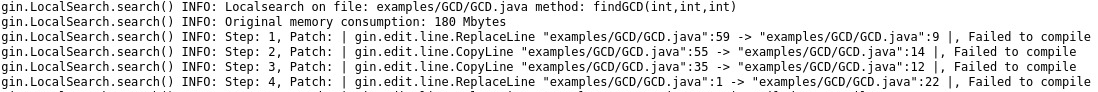
\includegraphics[width=1\textwidth]{img/GCD_MC_1.png}
  %\caption{Command line output: Memory Consumption Optimized GCD Java program with Gin tool.}
  %\label{fig:GCD_MC_1}
%\end{figure}

%\vspace{1em}
%By examining the output in figure \ref{fig:GCD_MC_2}, we were able to identify the specific patches that led to successfully compiled code with improved memory consumption performance. Our primary objective was to identify the best patch that consumed the least memory while passing all provided tests. In summary, the optimization results indicate the best memory consumption at 28 Mbytes, representing a reduction of 84.44\%.

%\begin{figure}[htbp]
  %\centering
  %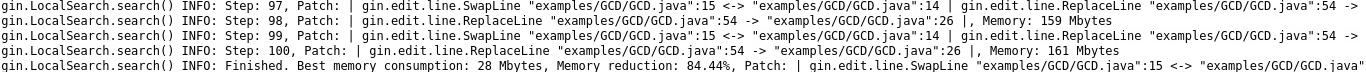
\includegraphics[width=1\textwidth]{img/GCD_MC_2.png}
  %\caption{Command line output: Memory Consumption Optimized GCD Java program with Gin tool.}
  %\label{fig:GCD_MC_2}
%\end{figure}

%\vspace{1em}
%Finally, in the same directory where the original GCD program is, the optimized code of GCD program for memory consumption was generated based on the best patch that consumed the lowest memory.

%\subsubsection{Multi criteria Fitness: Combined Execution time and Memory consumption}
%In our experiment, we aimed to optimize both the execution time and memory consumption together of the ‘findGCD’ method in the ‘GCD’ Java program using Gin’s local search algorithm. As Gin’s default ‘LocalSearch’ Java class was primarily designed for execution time minimization, we adapted it to minimize both execution time and memory consumption together. The updated version of the class can be accessed at the provided \href{https://gitlabev.imtbs-tsp.eu/sticamsud/enact-internship-2023/-/blob/main/Code/gin/Version_three_ExecutionTime_and_MemoryConsumption/gin/src/main/java/gin/LocalSearch.java}{link}. The LocalSearch class has been refined to optimize both memory consumption and execution time for patches. To achieve this, a unique scoring system was devised where both the execution time and memory usage for each patch are normalized and summed. This aggregated score acts as the objective function, with the goal being its minimization. Consequently, a lower score indicates better performance in terms of time and memory. Throughout its iterations, the LocalSearch class tests various patches on the source code, selecting and retaining the one that produces the lowest score, thus ensuring efficient code performance. Our experimental procedures followed the same procedures as single-criteria fitness for execution time

%\subsubsection{Experimental Results and Analysis:}

%In this section, we detail the optimization results for the "findGCD" method in the GCD Java program, specifically focusing on execution time and memory consumption together. Using the Gin tool, the experiment showed that the method's Original execution time: 2892005383 ns and Original memory usage was 158 Mbytes, as seen in figure \ref{fig:GCD_EC_MC_1}.

%\begin{figure}[htbp]
  %\centering
  %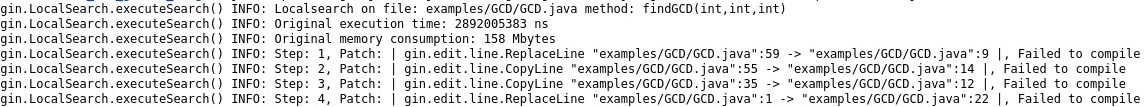
\includegraphics[width=1\textwidth]{img/GCD_ET_MC_1.png}
  %\caption{Command line output: Combined Execution time and Memory Consumption Optimized GCD Java program with Gin tool.}
 %\label{fig:GCD_EC_MC_1}
%\end{figure}

%By analyzing the output in figure \ref{fig:GCD_EC_MC_2}, we identified specific patches that resulted in a successful code compilation and enhanced both execution time and memory consumption performance. Our main goal was to find the most optimal patch one that sped up the program and consumed the least memory while still passing all the tests. In summary, the optimization results indicate the Best time: 2631710897 (ns), Speedup (\%): 9.00, Best memory consumption: 23 Mbytes, Memory reduction: 85.44\%.

%\begin{figure}[htbp]
  %\centering
  %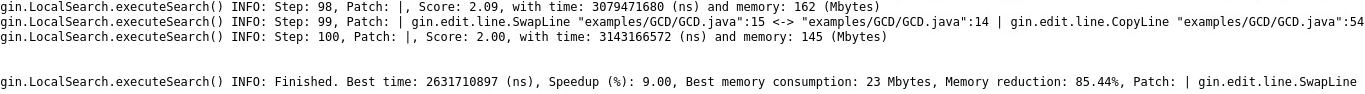
\includegraphics[width=1\textwidth]{img/GCD_ET_MC_2.png}
  %\caption{Command line output: Combined Execution time and Memory Consumption Optimized GCD Java program with Gin tool.}
  %\label{fig:GCD_EC_MC_2}
%\end{figure}

%\vspace{1em}
%Finally, in the same directory where the original GCD program is, the optimized code of GCD program for execution time and memory consumption together was generated. This optimization was based on the best patch, which yielded the lowest memory consumption and shortest execution time.



%\subsection{Rectangle Program Optimization using Gin Tool}

%In this section, we describe our experimental process, wherein we sought to optimize the "Rectangle" Java program. Specifically, our goal was to enhance the performance of the "classifyRectangle" method within this program. We targeted three distinct fitness criteria: two single criteria fitness "Execution Time," "Memory Consumption," and a multi-criteria fitness, "Combined Execution Time and Memory Consumption."

%\vspace{.5em}
%To begin the experiment, we selected the "Rectangle\footnote{\url{https://gitlabev.imtbs-tsp.eu/sticamsud/enact-internship-2023/-/blob/main/Code/gin/Version_one_Execution_Time/gin/examples/rectangle/Rectangle.java}}" program as our target.  The Rectangle program classifies a quadrilateral using its four side lengths into either a square, rectangle or an invalid shape. It deems the shape as a square if all sides are equal, a rectangle if opposite sides are identical, and invalid if any side is non-positive or if the sides don't conform to either the square or rectangle criteria. Our three experiments are grounded in the fitness criteria mentioned earlier. The ultimate objective was to enhance the program's efficiency, minimizing execution time, memory consumption, and the combination of both. We applied Gin's local search algorithm to achieve this. 


%\subsubsection{Single criteria Fitness: Execution time}
%In this experiment, our objective was to enhance the performance of the "classifyRectangle" method within the "Rectangle" Java program. Our primary focus was to minimize its execution time. To achieve this, the program was executed using a specified command, and we applied Gin’s local search algorithm.

%\subsubsection{Experimental procedures}
%\begin{enumerate}

%\item \textbf{Prerequisites:} Gin requires:
%\begin{itemize}
%\item JDK 17
%\item Gradle (tested with version 8.0.2)
%\item A number of dependencies, which can be downloaded manually or via Gradle (recommended)
%\item For Maven projects: make sure the Java version is set to the same version as Gin's.
%\end{itemize}

%\item \textbf{Clone the Repository:} Start by cloning the repository using the following command:

%\begin{verbatim}
%git clone https://github.com/gintool/gin.git
%\end{verbatim}

%\item \textbf{Navigate to the examples Directory:} Change the directory to the project folder:
%\begin{verbatim}
%cd gin/examples/rectangle
%\end{verbatim}

%\item \textbf{Compile the RectangleTest.java file:} Compile the RectangleTest.java program by running the following command:
%\begin{verbatim}
%javac -cp /usr/share/java/junit4.jar:. RectangleTest.java
%\end{verbatim}

%\item \textbf{Navigate to the gin Directory:} Change the directory to the gin folder:
%\begin{verbatim}
%cd ../../
%\end{verbatim}

%\item \textbf{Build using gradle (alternatively import into any IDE, such as IntelliJ) :}
%\begin{verbatim}
%gradle build
%\end{verbatim}

%This will build and test Gin, and also create a fat jar at build/gin.jar containing all required dependencies.

%Note: If the provided build command will not work use the following command below:
%\begin{verbatim}
%./gradlew clean build -x test copyToLib
%\end{verbatim}

%This will ensure a clean build by removing any existing build artifacts, compiles the source code, skips test execution, and then executes the custom copyToLib task, which carries out additional project-specific actions defined in the build script and also create a fat jar at build/gin.jar containing all required dependencies.


%\item \textbf{Execute (running Gin's local search on a simple example) by running the following command:}
%\begin{verbatim}
%java -jar build/gin.jar -f examples/triangle/Rectangle.java -m 
%"classifyRectangle(int,int,int,int)"
%\end{verbatim}

%Note: If the provided command for Running a Simple Example will not able to work, follow the below informations and execute the commands:
%\begin{verbatim}
%java -cp build/gin.jar:lib/junit-vintage-engine-5.9.2.jar gin.LocalSearch -f
%examples/rectangle/Rectangle.java -m "classifyRectangle(int,int,int,int)"
%\end{verbatim}
%Note: In this command specified the location of the necessary JAR files.
%\end{enumerate}

%\subsubsection{Experimental Results and Analysis:}

%This section presents the experimental results and analysis of the optimization experiment conducted to achieve an optimized Rectangle Java program. The focus of the optimization was specifically on improving the "classifyRectangle" method within the program, utilizing the Gin tool.

%\vspace{6em}
%\begin{figure}[htbp]
  %\centering
 % 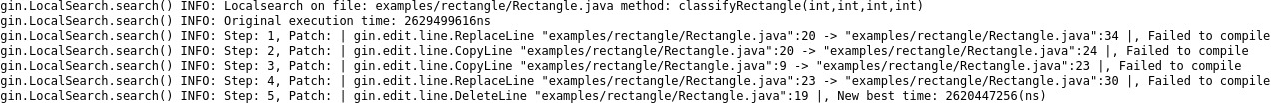
\includegraphics[width=1.\textwidth]{img/Rectangle_ET_1.png}
 % \caption{Command line output:Execution time Optimized %Rectangle Java program with Gin tool.}
 % \label{fig:Rectangle_ET_1}
%\end{figure}

%The output(figure \ref{fig:Rectangle_ET_1}) of the program provided information about each step of the local search process. It started with a summary of the file and method being analyzed, followed by reporting the original execution time of the method.The  Original execution time was 2629499616 ns.

%\begin{figure}[htbp]
  %\centering
  %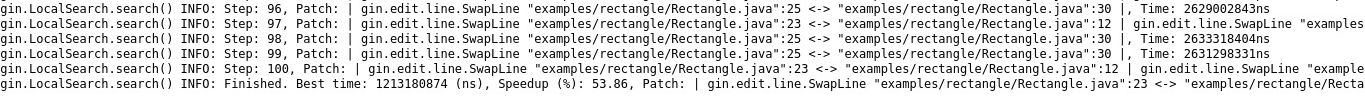
\includegraphics[width=1.\textwidth]{img/Rectangle_ET_2.png}
  %\caption{Command line output:Execution time Optimized %%Rectangle Java program with Gin tool.}
  %\label{fig:Rectangle_ET_2}
%\end{figure}
%
%By examining the output(figure \ref{fig:Rectangle_ET_2}), we could able to identify the patches that resulted in successfully compiled code and improved execution time performance. The goal was to find the fastest code that passed all provided tests. At the end of the process, a brief summary was provided to give an overview of the optimization results. Best time(Lowest execution time):1213180874 (ns), Speedup (\%): 53.86.

%\begin{figure}[htbp]
  %\centering
  %
\includegraphics[width=.7\textwidth]{img/Rectangle_ET_3.png}
  %\caption{Optimised program file of Rectangle program}
 % \label{fig:Optimised program file of Rectangle program}
%\end{figure}


%In Figure \ref{fig:Optimised program file of Rectangle program}, the directory where the optimized code was generated is specified. The figure displays the Optimised program file of the Rectangle program in blue, representing the code that has been improved for better performance. Conversely, the green color represents the original program file of the Rectangle program, which is the code in its initial state without any optimization. This color distinction helps visually differentiate between the optimized and original versions of the code.

%\subsubsection{Single criteria Fitness: Memory Consumption}

%In our experiment, we aimed to optimize the memory consumption of the ``classifyRectangle'' method in the ``Rectangle'' Java program using Gin's local search algorithm. Gin's default \texttt{LocalSearch} Java class was primarily designed for execution time minimization. Given our specific objective of memory consumption minimization, as we made modifications previously to the \texttt{LocalSearch} class. The updated version of the class can be accessed at the \href{https://gitlabev.imtbs-tsp.eu/sticamsud/enact-internship-2023/-/blob/main/Code/gin/Version_two_Memory_Consumption/gin/src/main/java/gin/LocalSearch.java}{link}. Our experimental procedures followed the same experimental procedures of single-criteria fitness: execution time.

%\subsubsection{Experimental Results and Analysis:}
%In this section, we detail the optimization results for the "classifyRectangle" method in the Rectangle Java program, specifically focusing on memory consumption. Using the Gin tool, the experiment showed that the method's original memory usage was 26 Mbytes, as seen in figure \ref{fig:Rectangle_MC_1}.

%\begin{figure}[htbp]
  %\centering
  %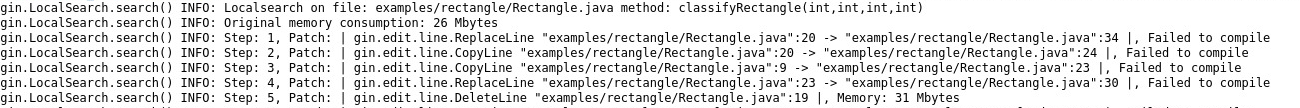
\includegraphics[width=1\textwidth]{img/Rectangle_MC_1.png}
  %\caption{Command line output: Memory Consumption Optimized %Rectangle Java program with Gin tool.}
  %\label{fig:Rectangle_MC_1}
%\end{figure}

%\vspace{1em}
%By examining the output in figure \ref{fig:Rectangle_MC_2}, we were able to identify the specific patches that led to successfully compiled code with improved memory consumption performance. Our primary objective was to identify the best patch that consumed the least memory while passing all provided tests. In summary, the optimization results indicate the best memory consumption at 14 Mbytes, representing a reduction of 46.15\%.

%\begin{figure}[htbp]
  %\centering
  %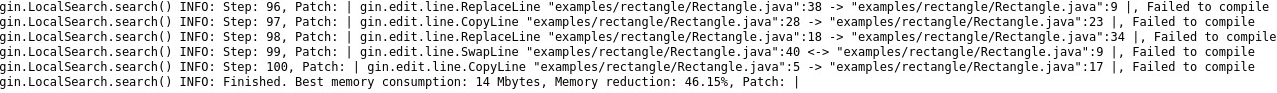
\includegraphics[width=1\textwidth]{img/Rectangle_MC_2.png}
  %\caption{Command line output: Memory Consumption Optimized Rectangle Java program with Gin tool.}
  %\label{fig:Rectangle_MC_2}
%\end{figure}

%\vspace{1em}
%Finally, in the same directory where the original Rectangle program is, the optimized code of Rectangle program for memory consumption was generated based on the best patch that consumed the lowest memory.

%\subsubsection{Multi criteria Fitness: Combined Execution time and Memory consumption}
%In our experiment, we aimed to optimize both the execution time and memory consumption together of the ‘classifyRectangle’ method in the ‘Rectangle’ Java program using Gin’s local search algorithm. As Gin’s default ‘LocalSearch’ Java class was primarily designed for execution time minimization, we adapted it to minimize both execution time and memory consumption together. The updated version of the class can be accessed at the provided \href{https://gitlabev.imtbs-tsp.eu/sticamsud/enact-internship-2023/-/blob/main/Code/gin/Version_three_ExecutionTime_and_MemoryConsumption/gin/src/main/java/gin/LocalSearch.java}{link}. The LocalSearch class has been refined to optimize both memory consumption and execution time for patches. Our experimental procedures followed the same procedures as single-criteria fitness for execution time

%\subsubsection{Experimental Results and Analysis:}

%In this section, we detail the optimization results for the "classifyRectangle" method in the Rectangle Java program, specifically focusing on execution time and memory consumption together. Using the Gin tool, the experiment showed that the method's Original execution time: 2707476462 ns and Original memory usage was 31 Mbytes, as seen in figure \ref{fig:Rectangle_EC_MC_1}.

%\begin{figure}[htbp]
  %\centering
  %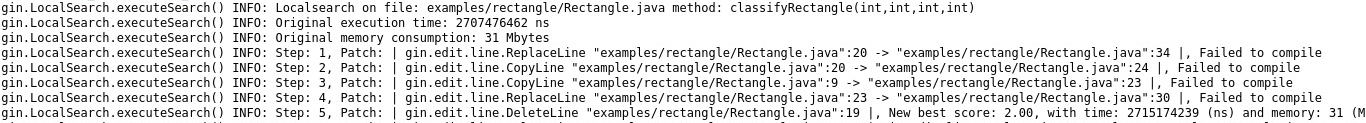
\includegraphics[width=1\textwidth]{img/Rectangle_ET_MC_1.png}
  %\caption{Command line output: Combined Execution time and Memory Consumption Optimized Rectangle Java program with Gin tool.}
  %\label{fig:Rectangle_EC_MC_1}
%\end{figure}

%By analyzing the output in figure \ref{fig:Rectangle_EC_MC_2}, we identified specific patches that resulted in a successful code compilation and enhanced both execution time and memory consumption performance. Our main goal was to find the most optimal patch one that sped up the program and consumed the least memory while still passing all the tests. In summary, the optimization results indicate the Best time: 1286266785  (ns), Speedup (\%): 52.49, Best memory consumption: 20 Mbytes, Memory reduction:35.48\%.

%\begin{figure}[htbp]
  %\centering
 % 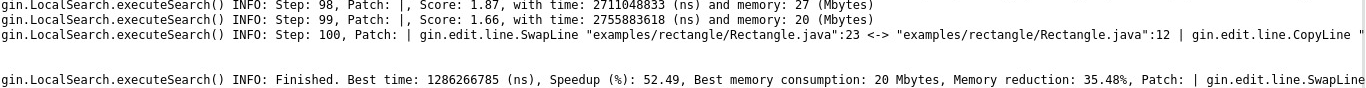
\includegraphics[width=1\textwidth]{img/Rectangle_ET_MC_2.png}
  %\caption{Command line output: Combined Execution time and Memory Consumption Optimized Rectangle Java program with Gin tool.}
 % \label{fig:Rectangle_EC_MC_2}
%\end{figure}

%\vspace{1em}
%Finally, in the same directory where the original Rectangle program is, the optimized code of Rectangle program for execution time and memory consumption together was generated. This optimization was based on the best patch, which yielded the lowest memory consumption and shortest execution time.

\vspace{-10pt}
\section{Experimental Results using JoularJX }

%\subsection{Experimental executions using JoularJX for optimised program based on the best patch given by Gin}

In the previous section, we obtained the optimization of selected programs (\ie \textit{Triangle}, \textit{GCD}, \textit{Rectangle}) using the Gin toolbox. 
%This optimization was based on single-criteria fitness (either Execution Time or Memory Consumption) and multi-criteria fitness (combining both Execution Time and Memory Consumption).  
In this section, 
%This analysis aims to 
we aim to answer our research question \textbf{RQ:2.1} (\ie \textit{Does the improvement of execution time and memory consumption reduce energy consumption?}). 

\vspace{.5em}
To do that, we first collected energy consumption measurements of the executions of the two versions, \ie original and optimised versions, of the studied programs. This was done by using \textit{JoularJX}. For this, we reused the same experimental procedures introduced in our preliminary study (\ie Section~\ref{subsec: mandelbrot java program} that details the monitoring of the energy consumed by a single program), and made modifications to the script (the \texttt{jx\_script.sh} is presented in Appendix~\ref{sec:mainscript}) to adapt it to the studied programs. 
These procedures were followed for each original and optimized version of the selected programs to monitor their energy consumption. 
%For this, we reuse and adapt the scripts used in our preliminary study (the \texttt{jx_script.sh} is presented in Appendix~\ref{sec:mainscript}). 
We then use the \texttt{Wilcoxon} statistical test to determine any significance difference of the consumed energy of the versions of the studied programs.  


%we detail our process for monitoring the energy consumption of both the original and the optimized versions of the programs using the \textit{JoulerJX} tool. We then use the \texttt{Wilcoxon} test to determine any significance difference of the consumed energy of the versions of the programs.  
%compare the energy consumption data of both versions and determine whether the optimized versions consume less energy than their original version. 
%This analysis aims to answer our research question  \textbf{RQ:2.1} (\ie \textit{Does the improvement of execution time and memory consumption reduce energy consumption?}).

\vspace{0.5em}

%After obtaining the optimized versions of the selected programs, we created two folders: one for the original versions and another for the optimized ones. In each folder, we incorporated all necessary scripts to monitor energy consumption using joularjx.
%As detailed in subsection \ref{subsec: mandelbrot java program} regarding monitoring the energy consumption of a single program, we adhered to the same experimental procedures. We made modifications to the script based on the program's name and class path. These procedures were followed for each original and optimized version of the selected programs to monitor their energy consumption. 

\vspace{0.5em}
For the energy consumption monitoring, we executed 30 times each version of each studied program using the previous script, it means that we isolated each monitoring. For instance, for evaluating the effect of the \textbf{Tactic 1}, \ie minimizing execution time, we first monitored the energy consumption of the original version of the \textit{Triangle} program. Then, we monitored the energy consumption of the optimized version for \textit{Triangle} program.
Finally, we compared collected data to evaluate if there is any significance difference between them.
We repeat the same process for the other tactic, \ie \textbf{Tactic 2} - \textit{minimizing memory consumption} and \textbf{Tactic 3} - \textit{minimizing execution time and memory consumption}, and for the others programs, \ie the \textit{GCD} and the \textit{Rectangle} programs.
%of the \textit{Triangle} program, again for a single fitness criterion: execution time.
%For each energy monitoring experiment, we ran two versions of each program: the original and the optimized version. Each version was executed for 30 iterations, consistent with the method described in subsection \ref{subsec: mandelbrot java program}. I conducted each experiment in isolation. For instance, I first monitored the energy consumption for the original Triangle program for a single fitness criterion: execution time. Subsequently, I monitored the energy consumption of the optimized Triangle program, again for a single fitness criterion: execution time.

\vspace{.5em}
Table~\ref{tab:Result} summarises the results obtained after performing our experimental study. As we can observe, 
we introduce per each version of the studied programs (see Column 1) the values obtained for each tactics applied. These obtained values correspond to the fitness values that were optimised and the corresponding energy consumption. Notice that we calculated the difference between energy consumed by the two versions of the programs (see the energy consumption values in Columns 3, 5 and 7 of the optimised versions of programs in Rows 2, 4 and 6). 
Finally, we identify the best tactic to reduce energy consumption per program (see Column 8).

%\multicolumn{5}{c}{First Video}

{\footnotesize
\begin{longtable}{|p{1.15cm}|p{1.3cm}|p{1.8cm}|p{1.5cm}|p{1.8cm}|p{1.8cm}|p{1.8cm}|p{2.5cm}|}
  \hline
  \multirow{2}{1.1cm}{\textbf{Version of Program}} 
  & \multicolumn{2}{c|}{\textbf{Tactic 1: min ET}}
  & \multicolumn{2}{c|}{\textbf{Tactic 2: min MC}} 
  & \multicolumn{2}{c|}{\textbf{Tactic 3: min ET + MC}} 
  & \multirow{2}{2.5cm}{\textbf{Best Tactic for Reducing EC}}\\
  
  \cline{2-7}
   & \textbf{ET (s)}  & \textbf{EC (J)} 
  & \textbf{MC (Mbytes)} & \textbf{EC (J)} 
  & \textbf{ET + MC} & \textbf{EC (J)} & \\
  \hline
  
%  \cline{1-7}
   Original\par Triangle & 
   1.636\kern0.5em s &
   Mean:\kern0.1em 5.834\par \vspace{.5em} [Confidence Interval:95\% (5.391,\kern0.1em 6.276)]\par \vspace{.5em} SD:\kern0.1em 1.185\vspace{.5em} Relative SD:0.203 &
   28 Mbytes &
   Mean:\kern0.1em 7.241\par \vspace{.5em} [Confidence Interval:95\% (6.968,\kern0.1em  7.514)]\par \vspace{.5em} SD:0.731\vspace{.5em} Relative SD:0.100 &
   1.773 s\par \vspace{.5em} 30 Mbytes &
   Mean:\kern0.1em 8.282\par \vspace{.5em} [Confidence Interval:95\% (7.775,\kern0.1em  8.789)]\par \vspace{.5em} SD: 1.358\vspace{.5em} Relative SD:0.164 &
   \textbf{Tactic 3}: Execution\kern0.3em time,
   Memory Consumption\par\\
   
  \cline{1-7}
  Optimised\par Triangle & 
  1.616\kern0.5em s\par \vspace{1em} Speedup: 1.22\% &
  Mean:\kern0.1em 5.023\par \vspace{.5em} [Confidence Interval:95\% (4.579,\kern0.1em 5.467)]\par \vspace{.5em} SD:\kern0.1em 1.189\par \vspace{.5em} Relative SD:0.237\vspace{.5em} \textbf{Energy consumption reduction: $\sim13.9\%$} \vspace{.5em} &
  22 Mbytes\par \vspace{.5em} Memory reduction: 21.43\% &
  Mean:\kern0.1em 6.051\par \vspace{.5em} [Confidence Interval:95\% (5.738,\kern0.1em  6.365)]\par \vspace{.5em} SD: 0.839\par \vspace{.5em} Relative SD:0.138\vspace{.5em} \textbf{Energy consumption reduction: $\sim 16.43\%$}\vspace{.5em}&
  1.751 s\par Speedup: 1.22\%.\par \vspace{.5em}
  26 Mbytes\par Memory reduction: 13.33\% &
  Mean:\kern0.1em 5.955\par \vspace{.5em} [Confidence Interval:95\% (5.697,\kern0.1em  6.212)]\par \vspace{.5em} SD: 0.689\par \vspace{.5em} Relative SD:0.116\vspace{.5em} \textbf{Energy consumption reduction: $\sim 28.11\%$}\vspace{.5em} &
  \textbf{Energy consumption reduction: $\sim 28.11\%$}
  \\
  
  \hline
%  \cline{1-7}
   Original\par GCD & 
   2.813\kern0.5em s &
   Mean:\kern0.1em27.766\par \vspace{.5em} [Confidence Interval:95\% (26.889,\kern0.1em 28.643)]\par \vspace{.5em} SD:2.349\vspace{.5em} Relative SD:0.085 &
   180 Mbytes &
   Mean:\kern0.1em26.353\par \vspace{.5em} [Confidence Interval:95\% (25.537,\kern0.1em 27.169)]\par \vspace{.5em} SD:2.186\vspace{.5em} Relative SD:0.083 &
   2.892 s\par \vspace{.5em} 158 Mbytes &
   Mean:\kern0.1em26.747\par \vspace{.5em} [Confidence Interval:95\% (25.996,\kern0.1em 27.498)]\par \vspace{.5em} SD:2.011\vspace{.5em} Relative SD:0.075 &
   \textbf{Tactic 3}: Execution\kern0.3em time,
   Memory Consumption\par\\
  
  \cline{1-7}
  Optimised\par GCD & 
  2.462\kern0.5em s\par \vspace{.5em} Speedup: 12.48\% &
  Mean:\kern0.1em13.551\par \vspace{.5em} [Confidence Interval:95\% (13.103,\kern0.1em 13.999)]\par \vspace{.5em} SD: 1.199\par \vspace{.5em} Relative SD:0.088\vspace{.5em} \textbf{Energy consumption reduction: $\sim 51.16\%$}\vspace{.5em}  &
  28 Mbytes\par \vspace{1em} Memory reduction: 84.44\% &
  Mean:\kern0.1em12.848\par \vspace{.5em} [Confidence Interval:95\% (12.406,\kern0.1em 13.290)]\par \vspace{.5em} SD:1.184\par \vspace{.5em} Relative SD:0.092\vspace{.5em} \textbf{Energy consumption reduction: $\sim 51.26\%$}\vspace{.5em} &
  2.631 s\par Speedup: 9.00\%\par \vspace{.5em}
  23 Mbytes\par Memory reduction: 85.44\% &
  Mean:\kern0.1em12.964\par \vspace{.5em} [Confidence Interval:95\% (12.554,\kern0.1em 13.375)]\par \vspace{.5em} SD:1.099\par \vspace{.5em} Relative SD:0.084\vspace{.5em} \textbf{Energy consumption reduction: $\sim 51.53\%$}\vspace{.5em} & \textbf{Energy consumption reduction: $\sim 51.53\%$}\\
  
  
  \hline
%  \cline{1-7}
   Original\par Rectangle & 
   2.629\kern0.5em s &
   Mean:\kern0.1em 6.587\par \vspace{.5em} [Confidence Interval:95\% (6.027,\kern0.1em 7.147)]\par \vspace{.5em} SD:1.499\vspace{.5em} Relative SD:0.227  &
   26 Mbytes &
   Mean:\kern0.1em 6.431\par \vspace{.5em} [Confidence Interval:95\% (5.781,\kern0.1em 7.081)]\par \vspace{.5em} SD:1.741\vspace{.5em} Relative SD:0.270 &
   2.707 s\par \vspace{.5em} 31 Mbytes &
   Mean:\kern0.1em 7.411\par \vspace{.5em} [Confidence Interval:95\% (6.926,\kern0.1em 7.895)]\par \vspace{.5em} SD:1.297\vspace{.5em} Relative SD:0.175 & 
   \textbf{Tactic 1}: Execution Time \\
   
  
  \cline{1-7}
  Optimised\par Rectangle & 
  1.213\kern0.5em s\par \vspace{.5em} Speedup: 53.86\% &
  Mean:\kern0.1em 5.217\par \vspace{.5em} [Confidence Interval:95\% (4.908,\kern0.1em 5.527)]\par \vspace{.5em} SD:0.828\par \vspace{.5em} Relative SD:0.158\vspace{.5em} \textbf{Energy consumption reduction: $\sim 20.78\%$}\vspace{.5em} &
  14 Mbytes\par \vspace{1em} Memory reduction: 46.15\% &
  Mean:\kern0.1em 5.299\par \vspace{.5em} [Confidence Interval:95\% (4.705,\kern0.1em 5.895)]\par \vspace{.5em} SD:1.594\par \vspace{.5em} Relative SD:0.300\vspace{.5em} \textbf{Energy consumption reduction: $\sim 17.6\%$}\vspace{.5em} &
  1.286 s\par Speedup: 52.59\%\par \vspace{1em}
  20 Mbytes\par Memory reduction: 35.48\% &
  Mean:\kern0.1em 6.340\par \vspace{.5em} [Confidence Interval:95\% (5.815,\kern0.1em 6.866)]\par \vspace{.5em} SD:1.407\par \vspace{.5em} Relative SD:0.221\vspace{.5em} \textbf{Energy consumption reduction: $\sim 14.45\%$}\vspace{.5em} &
  \textbf{Energy consumption reduction: $\sim 20.78\%$}
  \\
  
  
 \hline
\caption{Comparison of the energy consumed by the original vs. the optimized versions of the studied programs, \textit{where: ET=execution time in seconds, MC=memory consumption in Megabytes, EC=energy consumption in Joules}}
\label{tab:Result}
\end{longtable}
}
%Comparison between Single criteria fitness(Execution Time, Memory Consumption individually) and Multi criteria fitness(Execution Time, Memory Consumption combine).

\vspace{.5em}
In the following sections we provide the analysis of our results per program and then we discuss the results to get some general conclusions of this study.

\vspace{-5pt}
\subsection{Energy Consumption comparison for the original vs. the optimized versions of the \textit{Triangle} Program}

As we can observe in Table~\ref{tab:Result}, the Gin toolbox was able to optimised the \textit{Triangle} program by using \textbf{Tactic 1 - minimizing the execution time}. The obtained execution time was 1.636 seconds for the original version and 1.616 seconds for the optimised version, thus reducing 1.22\% of execution time (see Column 2 of Rows 1, 2) by applying Tactic 1. 
Regarding energy consumption, we obtained 5.834 joules for the original version and we obtained 5.023 joules for the optimised version. Thus, the energy consumption was reduced in 13.9\% by the optimised program (see Column 3 of Rows 1, 2) by applying Tactic 1.  
We can also observe this reduction of energy consumption in Figures~\ref{fig:triangle_tactic1_1} and~\ref{fig:triangle_tactic1_2} that shows the histogram and the box-plot of the data collected from 30 executions. Notice that the reported energy consumption are the mean values of energy consumption measurements collected from 30 executions. All of these mean values have confident error margin, \ie the relative standard deviation or coefficient of variance was lower than 5\%.


\begin{figure}
\centering
\subfigure[\textbf{Tactic 1} - Original vs. Optimized Triangle Histogram ]{
\label{fig:triangle_tactic1_1}
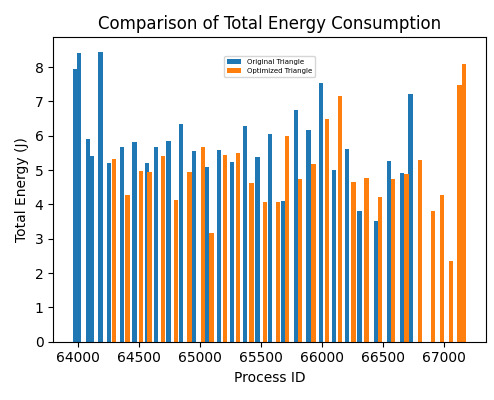
\includegraphics[width=0.45\textwidth,height=.3\textheight]{img/Triangle_ET_Comparision_histogram.png}
}
\subfigure[\textbf{Tactic 1} - Original vs. Optimized Triangle Boxplot]{
\label{fig:triangle_tactic1_2}
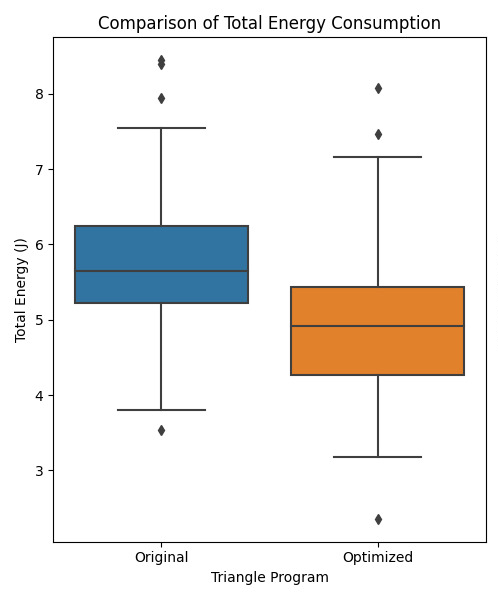
\includegraphics[width=0.47\textwidth,height=.3\textheight]{img/Triangle_ET_Comparision_boxplot.png}
}
\subfigure[\textbf{Tactic 2} - Original vs. Optimized Triangle Histogram]{
\label{fig:triangle_tactic2_1}
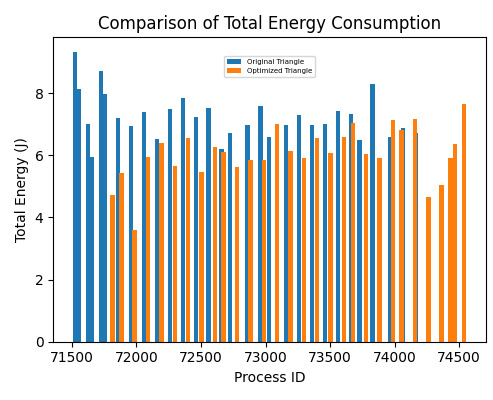
\includegraphics[width=0.45\textwidth,height=.3\textheight]{img/Triangle_MC_Comparision_histogram.png}
}
\subfigure[\textbf{Tactic 2} - Original vs. Optimized Triangle Boxplot]{
\label{fig:triangle_tactic2_2}
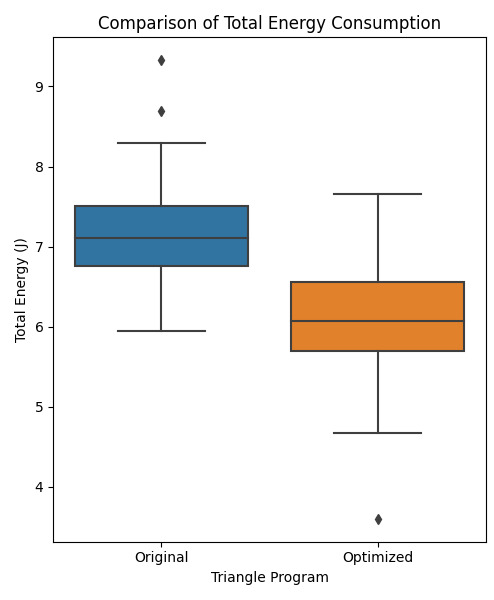
\includegraphics[width=0.47\textwidth,height=.3\textheight]{img/Triangle_MC_Comparision_boxplot.png}
}
\subfigure[\textbf{Tactic 3} - Original vs. Optimized Triangle Histogram]{
\label{fig:triangle_tactic3_1}
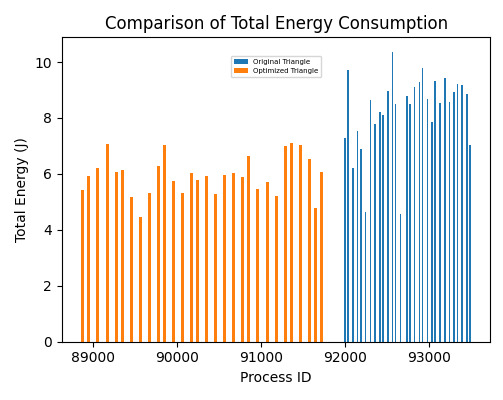
\includegraphics[width=0.45\textwidth,height=.3\textheight]{img/Trinagle_ET_MC_Comparison_histo.png}
} 
\subfigure[\textbf{Tactic 3} - Original vs. Optimized Triangle Boxplot]{
\label{fig:triangle_tactic3_2}
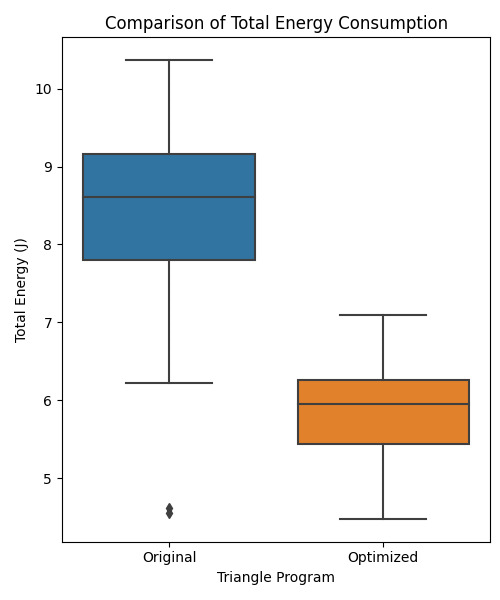
\includegraphics[width=0.47\textwidth,height=.3\textheight]{img/Trinagle_ET_MC_Comparison_box.png}
}
\caption{Energy consumption comparison for the original vs. optimized versions of the \textit{Triangle} program by applying the three studied tactics}
\label{fig:graphsTriangle}
\end{figure}

\vspace{.5em}
Moreover, the Gin toolbox was able to optimised the \textit{Triangle} program by using \textbf{Tactic 2 - minimizing the memory consumption}. The obtained memory consumption was 28 megabytes for the original version and 22 megabytes for the optimised version, thus reducing 21.43\% of memory consumption (see Column 4 of Rows 1, 2) by applying Tactic 2. 
Regarding energy consumption, we obtained 7.241 joules for the original version and we obtained 6.051 joules for the optimised version. Thus, the energy consumption was reduced in 16.43\% by the optimised program (see Column 5 of Rows 1, 2) by applying Tactic 2.
We can also observe this reduction of energy consumption in Figures~\ref{fig:triangle_tactic2_1} and~\ref{fig:triangle_tactic2_2} that shows the histogram and the box-plot of the data collected from 30 executions.

\vspace{.5em}
Finally, the Gin toolbox was able to optimised the \textit{Triangle} program by using \textbf{Tactic 3 - minimizing execution time and memory consumption}. The obtained fitness function was 1.773 seconds and 30 megabytes for the original version and 1.751 seconds and 26 megabytes for the optimised version, thus reducing 1.22\% of execution time and 13.33\% of memory consumption (see Column 6 of Rows 1, 2) by applying Tactic 3. 
Regarding energy consumption, we obtained 8.282 joules for the original version and we obtained 5.955 joules for the optimised version. Thus, the energy consumption was reduced in 28.11\% by the optimised program (see Column 7 of Rows 1, 2) by applying Tactic 3.  
We can also observe this reduction of energy consumption in Figures~\ref{fig:triangle_tactic3_1} and~\ref{fig:triangle_tactic3_2} that shows the histogram and the box-plot of the data collected from 30 executions.

\vspace{.5em}
We observe that for the \textit{Triangle} program the best tactic for reducing energy consumption was \textbf{Tactic 3 - minimizing execution time and memory consumption}. This tactic was able to reduce in 28.11\% the energy consumed by the  \textit{Triangle} program (see Column 8 of Rows 1, 2).

\vspace{.5em}
Notice that when a multi-criteria fitness function is used to optimise a code, each fitness value is optimised in a less percentage than optimising the code by using a single fitness function. For instance, while the percentage of the reduced execution time for Tactic 1 and Tactic 3 are equivalent, the percentage for the consumed memory was penalised from 21.43\% to 13.33\%. Instead of this penalisation, Tactic 3 is the most effective tactic to reduce energy consumption for the \textit{Triangle} program. It could be due to the energy consumed by programs does not only depends on execution time but also depends on the use of CPU. Therefore, if we optimise the memory consumption it could help to reduce the use of CPU, thus reducing energy consumption.

%In this subsection, we will detail the results of a comparison between two versions of the Triangle program (original and optimized) using the Wilcoxon test. Based on this analysis, we will determine which version of the Triangle program consumes more energy.  We have three optimized programs, each based on different criteria: Single criteria fitness: Execution time, Single criteria fitness: Memory consumption, Multi-criteria fitness: Combined execution time and memory consumption. For each fitness criterion, we first monitored the energy consumption of the original Triangle program, followed by its optimized version. We then compared the results using the Wilcoxon test. Because each experiment was conducted in isolation, the energy consumption of the original Triangle program varied with each fitness criterion.

\vspace{-5pt}
\subsection{Energy Consumption comparison for the original vs. the optimized versions of the \textit{Greatest Common Divisor(GCD)} Program}

As we can observe in Table~\ref{tab:Result}, the Gin toolbox was able to optimised the \textit{Greatest Common Divisor(GCD)} program by using \textbf{Tactic 1 - minimizing the execution time}. The obtained execution time was 2.813 seconds for the original version and 2.462  seconds for the optimised version, thus reducing 12.48\% of execution time (see Column 2 of Rows 3, 4) by applying Tactic 1. 
Regarding energy consumption, we obtained 27.766 joules for the original version and we obtained 13.551 joules for the optimised version. Thus, the energy consumption was reduced in 51.16\% by the optimised program (see Column 3 of Rows 3, 4) by applying Tactic 1.  
We can also observe this reduction of energy consumption in Figures~\ref{fig:gcd_tactic1_1} and~\ref{fig:gcd_tactic1_2} that shows the histogram and the box-plot of the data collected from 30 executions.
Notice that the reported energy consumption are the mean values of energy consumption measurements collected from 30 executions. All of these mean values have confident error margin, \ie the relative standard deviation or coefficient of variance was lower than 5\%.


\begin{figure}
\centering
\subfigure[\textbf{Tactic 1} - Original vs. Optimized GCD Histogram]{
\label{fig:gcd_tactic1_1}
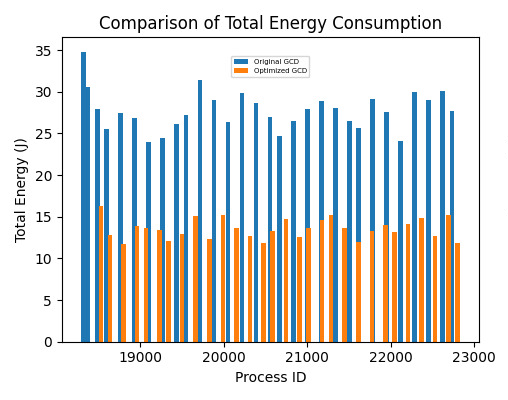
\includegraphics[width=0.45\textwidth,height=.3\textheight]{img/GCD_ET_Comparison_his.png}
}
\subfigure[\textbf{Tactic 1} - Original vs. Optimized GCD Boxplot]{
\label{fig:gcd_tactic1_2}
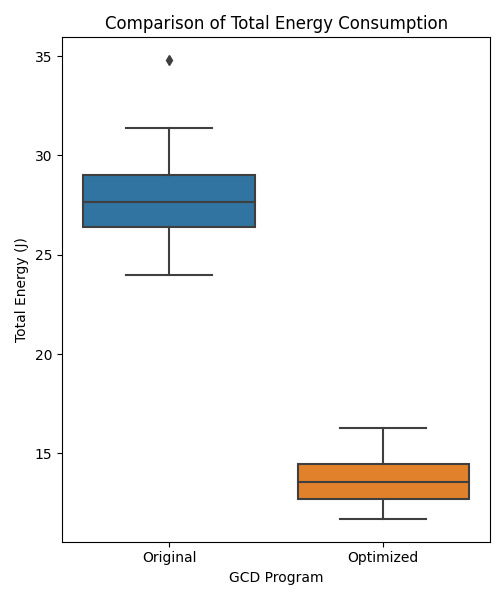
\includegraphics[width=0.47\textwidth,height=.3\textheight]{img/GCD_ET_Comparison_box.png}
}
\subfigure[\textbf{Tactic 2} - Original vs. Optimized GCD Histogram]{
\label{fig:gcd_tactic2_1}
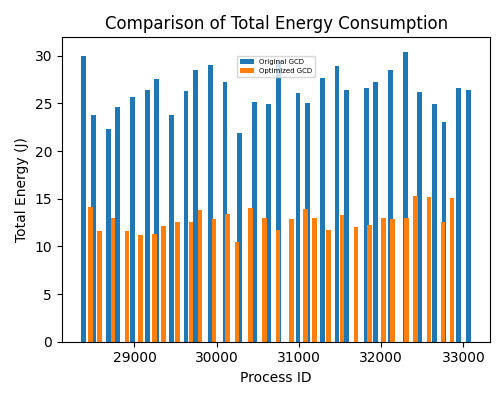
\includegraphics[width=0.45\textwidth,height=.3\textheight]{img/GCD_MC_his.png}
}
\subfigure[\textbf{Tactic 2} - Original vs. Optimized GCD Boxplot]{
\label{fig:gcd_tactic2_2}
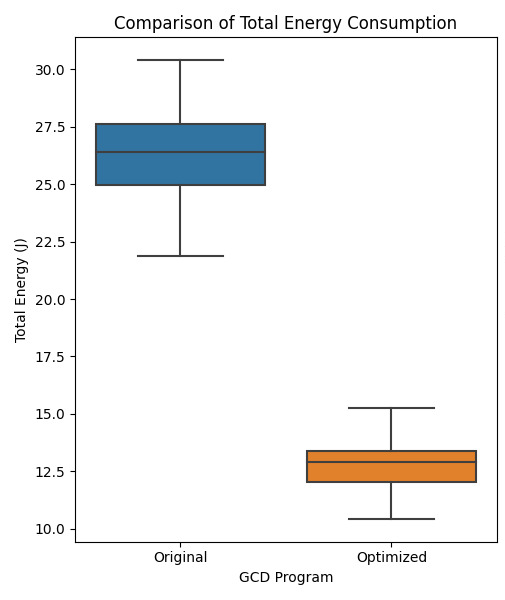
\includegraphics[width=0.47\textwidth,height=.3\textheight]{img/GCD_MC_box.png}
}
\subfigure[\textbf{Tactic 3} - Original vs. Optimized GCD Histogram]{
\label{fig:gcd_tactic3_1}
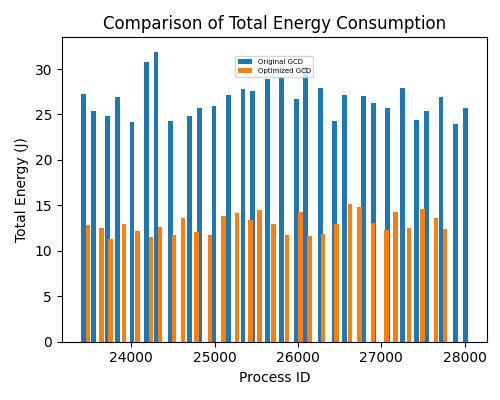
\includegraphics[width=0.45\textwidth,height=.3\textheight]{img/GCD_ET_MC_his.png}
} 
\subfigure[\textbf{Tactic 3} - Original vs. Optimized GCD Boxplot]{
\label{fig:gcd_tactic3_2}
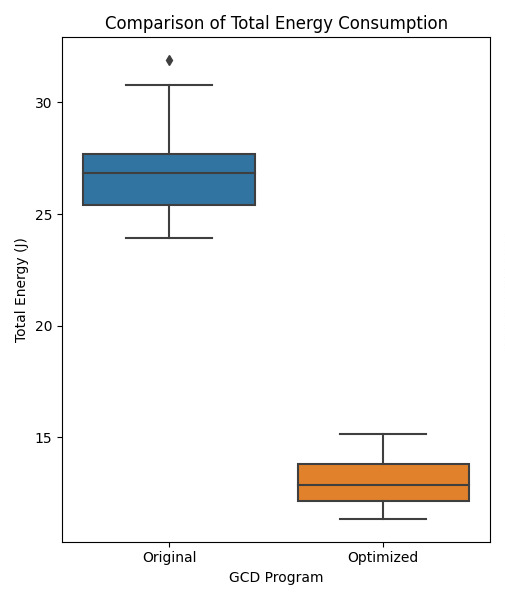
\includegraphics[width=0.47\textwidth,height=.3\textheight]{img/GCD_ET_MC_box.png}
}
\caption{Energy consumption comparison for the original vs. optimized versions of the \textit{Greatest Common Divisor(GCD)} program by applying the three studied tactics}
\label{fig:graphsGCD}
\end{figure}

\vspace{.5em}
Moreover, the Gin toolbox was able to optimised the \textit{Greatest Common Divisor(GCD)} program by using \textbf{Tactic 2 - minimizing the memory consumption}. The obtained memory consumption was 180 megabytes for the original version and 28 megabytes for the optimised version, thus reducing 84.44\% of memory consumption (see Column 4 of Rows 3, 4) by applying Tactic 2. Regarding energy consumption, we obtained 26.353 joules for the original version and we obtained 12.848 joules for the optimised version. Thus, the energy consumption was reduced in 51.26\% by the optimised program (see Column 5 of Rows 3, 4) by applying Tactic 2.
We can also observe this reduction of energy consumption in Figures~\ref{fig:gcd_tactic2_1} and~\ref{fig:gcd_tactic2_2} that shows the histogram and the box-plot of the data collected from 30 executions.

\vspace{.5em}
Finally, the Gin toolbox was able to optimised the \textit{Greatest Common Divisor(GCD)} program by using \textbf{Tactic 3 - minimizing execution time and memory consumption}. The obtained fitness function was 2.892 seconds and 158  megabytes for the original version and 2.631 seconds and 23 megabytes for the optimised version, thus reducing 9.00\% of execution time and 85.44\% of memory consumption (see Column 6 of Rows 3, 4) by applying Tactic 3. Regarding energy consumption, we obtained 26.747 joules for the original version and we obtained 12.964 joules for the optimised version. Thus, the energy consumption was reduced in 51.53\% by the optimised program (see Column 7 of Rows 3, 4) by applying Tactic 3. We can also observe this reduction of energy consumption in Figures~\ref{fig:gcd_tactic3_1} and~\ref{fig:gcd_tactic3_2} that shows the histogram and the box-plot of the data collected from 30 executions.

\vspace{.5em}
We observe that for the \textit{Greatest Common Divisor(GCD)} program the best tactic for reducing energy consumption was \textbf{Tactic 3 - minimizing execution time and memory consumption}. This tactic was able to reduce in 51.53\% the energy consumed by the  \textit{Greatest Common Divisor(GCD)} program (see Column 8 of Rows 3, 4).

\vspace{.5em}
Notice that when a multi-criteria fitness function is used to optimise a code, each fitness value is optimised in a less percentage than optimising the code by using a single fitness function. For instance, the percentage for the execution time was penalised from 12.48\% to 9.00\% in Tactic 1 to Tactic 3. Instead of this penalisation, Tactic 3 is the most effective tactic to reduce energy consumption for the \textit{Greatest Common Divisor(GCD)} program. It could be due to the energy consumed by programs does not only depends on execution time but also depends on the use of memory. Therefore, since Tactic 3 contains the highest memory reduce percentage it leads to reduction in energy consumption.

\vspace{-5pt}
\subsection{Energy Consumption comparison for the original vs. the optimized versions of the \textit{Rectangle} Program}

As we can observe in Table~\ref{tab:Result}, the Gin toolbox was able to optimised the \textit{Rectangle} program by using \textbf{Tactic 1 - minimizing the execution time}. The obtained execution time was 2.629 seconds for the original version and 1.213 seconds for the optimised version, thus reducing 53.86\% of execution time (see Column 2 of Rows 5, 6) by applying Tactic 1. 
Regarding energy consumption, we obtained 6.587 joules for the original version and we obtained 5.217 joules for the optimised version. Thus, the energy consumption was reduced in 20.78\% by the optimised program (see Column 3 of Rows 5, 6) by applying Tactic 1.  
We can also observe this reduction of energy consumption in Figures~\ref{fig:rectangle_tactic1_1} and~\ref{fig:rectangle_tactic1_2} that shows the histogram and the box-plot of the data collected from 30 executions.
Notice that the reported energy consumption are the mean values of energy consumption measurements collected from 30 executions. All of these mean values have confident error margin, \ie the relative standard deviation or coefficient of variance was lower than 5\%.



\begin{figure}
\centering
\subfigure[\textbf{Tactic 1} - Original vs. Optimized Rectangle Histogram]{
\label{fig:rectangle_tactic1_1}
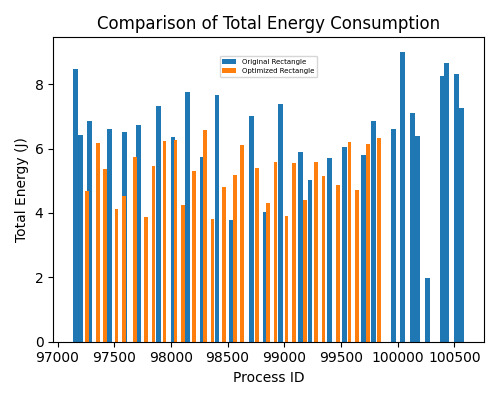
\includegraphics[width=0.45\textwidth,height=.3\textheight]{img/Rectangle_ET_comparison_his.png}
}
\subfigure[\textbf{Tactic 1} - Original vs. Optimized Rectangle Boxplot]{
\label{fig:rectangle_tactic1_2}
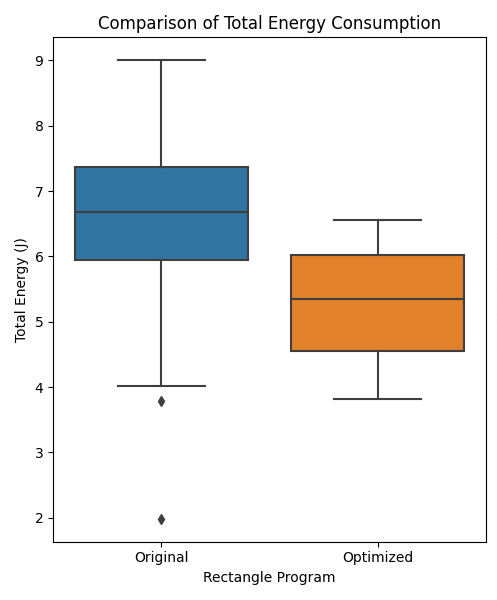
\includegraphics[width=0.47\textwidth,height=.3\textheight]{img/Rectangle_ET_Compariosn_box.png}
}
\subfigure[\textbf{Tactic 2} - Original vs. Optimized Rectangle Histogram]{
\label{fig:rectangle_tactic2_1}
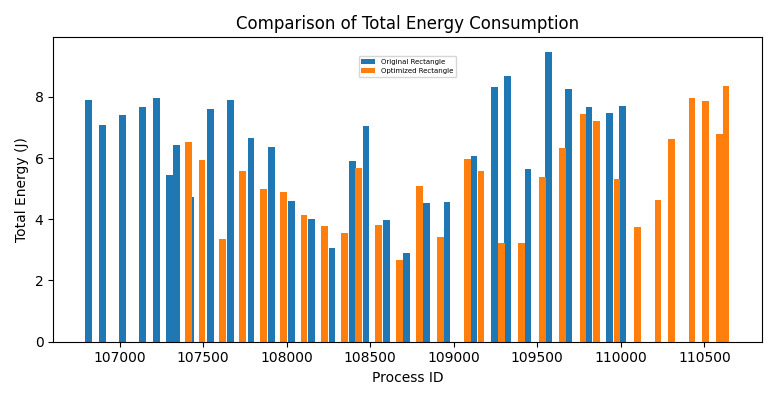
\includegraphics[width=0.45\textwidth,height=.3\textheight]{img/Rectangle_MC_Comparion_his.png}
}
\subfigure[\textbf{Tactic 2} - Original vs. Optimized Rectangle Boxplot]{
\label{fig:rectangle_tactic2_2}
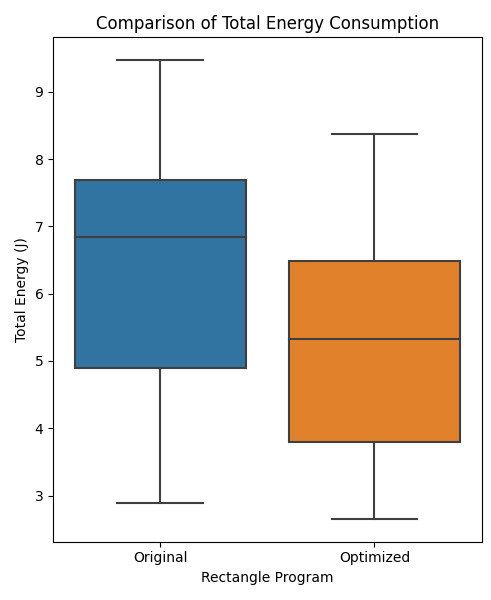
\includegraphics[width=0.47\textwidth,height=.3\textheight]{img/Rectangle_MC_Comparion_box.png}
}
\subfigure[\textbf{Tactic 3} - Original vs. Optimized Rectangle Histogram]{
\label{fig:rectangle_tactic3_1}
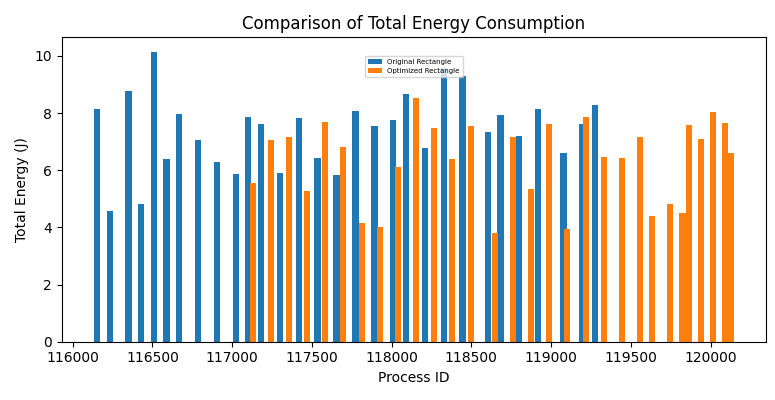
\includegraphics[width=0.45\textwidth,height=.3\textheight]{img/Rectangle_ET_MC_Comparion_his.png}
} 
\subfigure[\textbf{Tactic 3} - Original vs. Optimized Rectangle Boxplot]{
\label{fig:rectangle_tactic3_2}
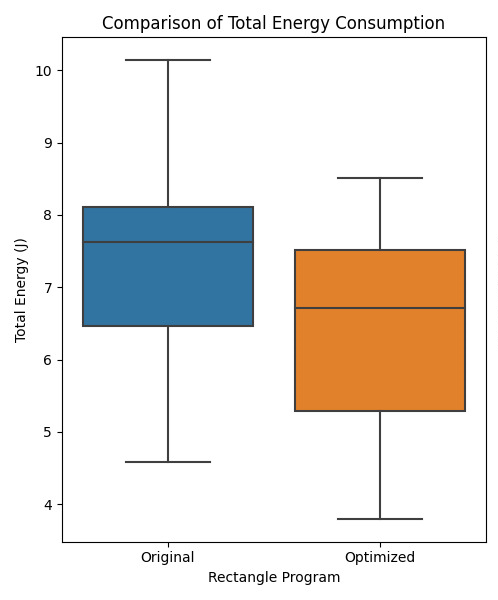
\includegraphics[width=0.47\textwidth,height=.3\textheight]{img/Rectangle_ET_MC_Comparion_Box.png}
}
\caption{Energy consumption comparison for the original vs. optimized versions of the \textit{Rectangle} program by applying the three studied tactics}
\label{fig:graphsRectangle}
\end{figure}

\vspace{.5em}
Moreover, the Gin toolbox was able to optimised the \textit{Rectangle} program by using \textbf{Tactic 2 - minimizing the memory consumption}. The obtained memory consumption was 26 megabytes for the original version and 14 megabytes for the optimised version, thus reducing 46.15\% of memory consumption (see Column 4 of Rows 5, 6) by applying Tactic 2. 
Regarding energy consumption, we obtained 6.431 joules for the original version and we obtained 5.299 joules for the optimised version. Thus, the energy consumption was reduced in 17.6\% by the optimised program (see Column 5 of Rows 5, 6) by applying Tactic 2.
We can also observe this reduction of energy consumption in Figures~\ref{fig:rectangle_tactic2_1} and~\ref{fig:rectangle_tactic2_2} that shows the histogram and the box-plot of the data collected from 30 executions.

\vspace{.5em}
Finally, the Gin toolbox was able to optimised the \textit{Rectangle} program by using \textbf{Tactic 3 - minimizing execution time and memory consumption}. The obtained fitness function was 2.707 seconds and 31 megabytes for the original version and 1.286 seconds and 20 megabytes for the optimised version, thus reducing 52.59\% of execution time and 35.48\% of memory consumption (see Column 6 of Rows 5, 6) by applying Tactic 3. Regarding energy consumption, we obtained 7.411 joules for the original version and we obtained 6.340 joules for the optimised version. Thus, the energy consumption was reduced in 14.45\% by the optimised program (see Column 7 of Rows 5, 6) by applying Tactic 3. We can also observe this reduction of energy consumption in Figures~\ref{fig:rectangle_tactic3_1} and~\ref{fig:rectangle_tactic3_2} that shows the histogram and the box-plot of the data collected from 30 executions.

\vspace{.5em}
We observe that for the \textit{Rectangle} program the best tactic for reducing energy consumption was \textbf{Tactic 1 - minimizing the execution time}. This tactic was able to reduce in 20.78\% the energy consumed by the  \textit{Triangle} program (see Column 8 of Rows 5, 6).

\vspace{-5pt}
\subsection{Discussion}

In Table~\ref{tab:Result}, we observe that the Gin toolbox was able to optimize the \textit{Triangle}, \textit{Greatest Common Divisor (GCD)}, and \textit{Rectangle} programs using \textbf{Tactic 1: minimizing the execution time}, \textbf{Tactic 2: minimizing memory consumption}, and \textbf{Tactic 3: minimizing execution time and memory consumption}, as discussed in Section \ref{sec:tactics}. Upon analyzing the table, we observed that the optimized version of each program consistently consumes less energy than its original version. We calculated the energy consumption reduction in percentage for each optimized version and then compared these percentages. 

\vspace{.5em}
For the \textit{Triangle} program, the energy consumption was reduced by 13.9\% with the optimized program when applying \textbf{Tactic 1} (see Column 3, Rows 1 and 2). With \textbf{Tactic 2}, the reduction was 16.43\% (see Column 5, Rows 1 and 2), and with \textbf{Tactic 3}, it was 28.11\% (see Column 7, Rows 1 and 2). We observe that, for the \textit{Triangle} program, \textbf{Tactic 3 - minimizing execution time and memory consumption} was the most effective, achieving a 28.11\% reduction in energy consumption (see Column 8, Rows 1 and 2).

\vspace{.5em}
For the \textit{Greatest Common Divisor (GCD)} program, the energy consumption was reduced by 51.16\% using the optimized program when applying \textbf{Tactic 1} (see Column 3, Rows 3 and 4). With \textbf{Tactic 2}, the reduction was 51.26\% (see Column 5, Rows 3 and 4), and with \textbf{Tactic 3}, it was 51.53\% (see Column 7, Rows 3 and 4). We observe that \textbf{Tactic 3 - minimizing execution time and memory consumption} was the most effective for the \textit{Greatest Common Divisor (GCD)} program, achieving a 51.53\% reduction in energy consumption (see Column 8, Rows 3 and 4).

\vspace{.5em}
For the \textit{Rectangle} program, the energy consumption was reduced by 20.78\% using the optimized program when applying \textbf{Tactic 1} (see Column 3, Rows 5 and 6). With \textbf{Tactic 2}, the reduction was 17.6\% (see Column 5, Rows 5 and 6), and with \textbf{Tactic 3}, it was 14.45\% (see Column 7, Rows 5 and 6). We observe that, for the \textit{Rectangle} program, \textbf{Tactic 1 - minimizing the execution time} was the most effective, achieving a 20.78\% reduction in energy consumption (see Column 8, Rows 5 and 6).

\vspace{.5em}
To definitively determine which tactic yields the highest energy consumption reduction, further experiments are needed. However, based on our current results, we can conclude that the optimized versions program using the "gin" tool, across all three tactics, consistently consume less energy than their original version program. This evidence supports a positive answer to research question \textbf{RQ2.1}: improvements in the execution time and memory consumption of programs do indeed lead to reduced energy consumption.